
%-----------------------------------------------------------------------------------
%-----------------------------------------------------------------------------------
%                                      PREAMBLE
%-----------------------------------------------------------------------------------
%-----------------------------------------------------------------------------------
\documentclass{article}
%-----------------------------------------------------------------------------------
% GENERIC PACKAGES
\usepackage[utf8]{inputenc}
\usepackage{graphicx}
\usepackage{hyperref}
\usepackage{setspace}
%-----------------------------------------------------------------------------------
% GEOMETRY
\usepackage{geometry}
\geometry{
    left=25mm,
    right=25mm,
    top=20mm,
    bottom=25mm
    }
\onehalfspacing
%-----------------------------------------------------------------------------------
% ACRONYMS
\usepackage{acro}
\DeclareAcronym{hri}{
  short=HRI,
  long=Human-Robot Interaction,
}
\DeclareAcronym{mis}{
  short=MIS,
  long=minimally Invasive Surgery,
}
\DeclareAcronym{ramis}{
  short=RAMIS,
  long=Robot-Assisted Minimally Invasive Surgery,
}
%-----------------------------------------------------------------------------------
% NEWCOMMANDS AND RENEWCOMMANDS

%-----------------------------------------------------------------------------------

% TITLE
\title{\textbf{Implementazione e valutazione di Vincoli Virtuali adattivi in formazione chirurgica con un robot chirurgico \textit{daVinci}: uno studio sperimentale}
\\
\vspace{0.5cm}\large{\textit{Alberto Rota} : NearLab @ Politecnico di Milano}
\\
\vspace{0.4cm}\small{Project Supervisor: \textit{prof. Elena De Momi}}
}
\author{}
\date{}

%-----------------------------------------------------------------------------------
%-----------------------------------------------------------------------------------
%                                      BODY
%-----------------------------------------------------------------------------------
%-----------------------------------------------------------------------------------
\begin{document}
% TITLE
\maketitle

%-----------------------------------------------------------------------------------
\section{Obiettivo}
Realizzare un simulatore per formazione chirurgica in ambiente virtuale che implementi Vincoli Virtuali aptici a fini correttivi, e valutare l'efficacia ed utilizzabilità di tali vincoli virtuali nel contesto di acquisizione, retenzione e trasferimento di abilità chirurgiche, 
% To implement a simulator for surgical training that employs haptic Virtual Fixtures as correction media, and to assess the effectiveness and utility of haptic Virtual Fixtures in the process of learning surgical skills, their retention and their transferability.

\paragraph*{Vincoli Virtuali Aptici}: 
Durante la tele-operazione di un robot chirurgico, i motori nei manipolatori vengono attivati cosicchè l'utilizzatore avverta una forza applicata alle sue mani: tale forza viene calcolata con l'obiettivo di redirezionare i movimenti del chirurgo lontano da ostacoli o verso obiettivi di interesse.
% When teleoperation the surgical robot, the motors in the manipulators are activated so that a force is felt by the surgeon: this force is applied with the aim of stirring the surgeon motion away from obstacles or towards objective
\paragraph*{Retenzione di abilità}: 
Dopo l'addestramento, l'aspirante chiruirgo dovrà essere in grado di tele-operare il robot correttamente anche dopo un periodo di tempo lontano dal simulatore.
% After surgical training, the trainee should be able to perform the surgical tasks correctly even after long periods of time away from the simulator
\paragraph*{Trasferimento di abilità}: 
Dopo l'addestramento, l'aspirante chiruirgo dovrà essere in grado di tele-operare il robot correttamente anche in situazioni non identiche a quelle su cui è stato formato.
% After surgical training conducted on a limited number of tasks, the trainee should be able to perform correctly on new never-seen-before chores.

\section{Progressi}
\begin{itemize}
  \item Il simulatore chirurgico è stato sviluppato con successo. La tele-operazione avviene tramite i manipolatori di un robot chirurgico \textit{daVinci}; le scene operatorie virtuali sono visibili in 3D dallo Stereo-Visore ad Alta Risoluzione alla console di teleoperazione.
  \item E' stato studiato un protocollo sperimentale, dove la performance di soggetti di studio (volontari) che riceveranno assistenza con Vincoli Virtuali verrà comparata con la performce di soggetti non-assistiti in un gruppo di controllo.
  \item Sono stati raccolti dati preliminari promettenti da una popolazione limitata (X soggetti) di volontari senza esperienza in chirurgia.  
  % \item  We successfully built the surgical training simulator. Teleoperation occurs from the manipulators of a \textit{daVinci} surgical robot; the virtual surgical scene is visible in 3D from the High-Resolution Stereo Viewers located at the teleoperation console
  % \item We have constructed a tentative experimental protocol, where the performance of volunteer subjects that will recieve haptic assistance will be compared with a control group where the assistance will not be provided.
  % \item We have gathered promising preliminary data from a very limited (X subject) population with no surgical experience
\end{itemize}

\section{Aspettative}
In a context where the subjects of the experimental study perform multiple times the surgical tasks over the course of a few days, and where the \textbf{performance} in the execution of a task is calculated as a numerical value, it is expected that:
\begin{itemize}
  \item Subjects in the assisted group will reach their best performances earlier than subjects in the control group
  \item The best performance of subjects in the assisted group will be higher than the best performance of subjects in the control group
  \item After a "break" of a few days, the subjects in the assisted group will be able to perform the surgical tasks with a performance comparable to the one obtained in the days before the break, \textit{i.e.} they will have \textbf{successfully retained their skill}
  \item After a "break" of a few days, the subjects in the assisted group will be able to perform new never-seen-before surgical tasks with a performance comparable to the one obtained in the days before the break, \textit{i.e.} they will \textbf{successfully have transferred their skill}
\end{itemize} 
The figure below shows graphically the expectations of the study

\begin{figure}[!h]
  \centering
  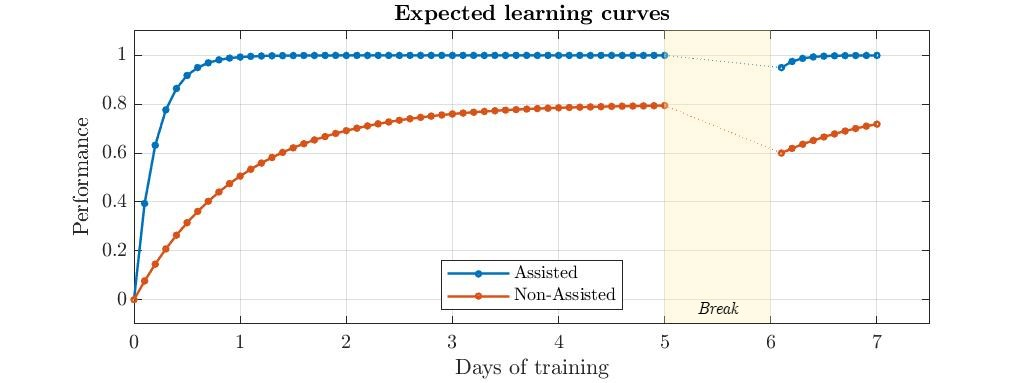
\includegraphics[width=0.85\textwidth]{expected.jpg}
  \end{figure} 
\section{Ulteriori requisiti}
Before proceeding with the experimental study, we must \textbf{assert the clinical relevance and compliance} of the surgical simulator that we have implemented and of the experimental protocol that we have planned. For that purpose opinions, corrections, criticism and involvement from the clinical community are encouraged and welcomed. 

\noindent We ask you to kindly dedicate approximately 30 minutes of your time to test the simulator (8 surgical tasks in total are implemented, each taking at the very maximum 1 minute) and to give us your feedback regarding the haptic Virtual Fixtures, the surgical simulator and the experimental protocol.

\section{Informazioni Aggiuntive}
Please contact Alberto at: \textit{\href{mailto:alberto2.rota@mail.polimi.it}{alberto2.rota@mail.polimi.it}} or \textit{+39 346 214 2633}
\newline Project Webpage: \href{https://github.com/alberto-rota/Virtual-Fixtures-in-Robotic-Assisted-Surgery}{https://github.com/alberto-rota/Virtual-Fixtures-in-Robotic-Assisted-Surgery} 


%-----------------------------------------------------------------------------------

\end{document}